\chapter{Keyboard Design} \label{keyboard_design}

\section{Word-Gesture Keyboard Implementation}
\subsection{Lacking Word-Recognition}
Recreating a word-gesture keyboard from scratch with the limited, non-commercial information available was outside the scope of this study. Word-recognition had already been proven to work and benefit word-gesture keyboards immensely \cite{ref_shape_writing,ref_the_word_gesture_keyboard,ref_shapewriter_iphone,ref_shark_wgk,ref_shorthand_writing}. In addition, the words that each participant was entering was known in advance; therefore, a pseudo word-gesture keyboard implementation was used.

\subsection{Design}
The pseudo word-gesture implementation was created by analyzing the gesture as it was being drawn to determine which keys were being pressed. The assumptions for detecting a key press were based off of the known word being gestured and noticeable deviations made in the gesture's direction. To reduce the chance of erroneous keys being produced, the sizes of the character that was expected to be pressed next were exaggerated and the threshold for detecting deviations in the gesture were lowered between keys.

The displayed keys were 64x64 pixels in size with a gap of 10 pixels between each key. The actual size of the keys was dependent on the display device being used. The next expected letter to be pressed in a word was changed into a circular key with a radius of 76.8 pixels, 20\% larger than the key widths, in order to make hitting keys even easier. Figure~\ref{key_bloating} shows how keys were changed behind the scenes; however, there was no feedback shown to the participant of the change in key size.

\begin{figure}[h]
	\centering
	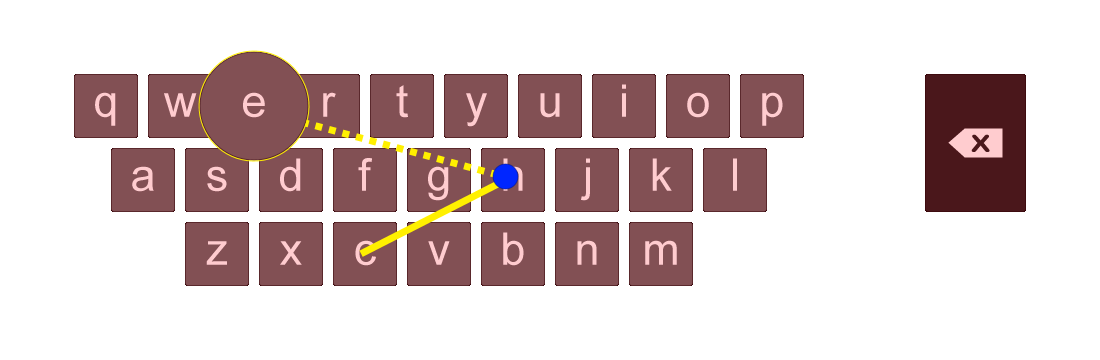
\includegraphics[width=5in]{fig_bloat_key}
	\caption[Larger Key Example]{Behind the scenes, invisible to the participant, the next key to be pushed is increased in size to make hitting it easier.}
	\label{key_bloating}
\end{figure}

An interpolated trail with points at a minimum of 16 pixels apart was used in determining deviations in word-gesturing. The angle of detecting a deviation was 165 degrees for all areas that were not on the expected path to the next key and was 90 degrees while on the expected path. Deviations in gesture path had to be at least 48 pixels away from each other to be detected. The expected path between two keys comprised an area from the previous expected key to the next expected key with a width 62.5\% larger than key size, or 104 pixels. Figure~\ref{protected_path} shows the how the expected path protects against natural deviations when moving from one key to the next.

\begin{figure}[h]
	\centering
	\begin{minipage}[t]{3in}
		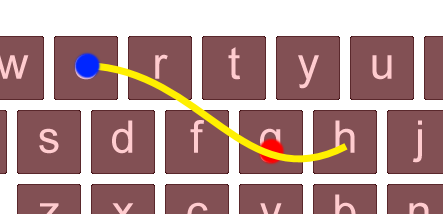
\includegraphics[width=2.5in]{fig_path_no_protection}
		\subcaption{No Path Protection\ \ \ \ \ \ \ \ \ }
	\end{minipage}
	\begin{minipage}[t]{2.5in}
		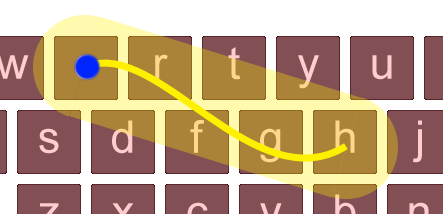
\includegraphics[width=2.5in]{fig_path_no_error}
		\subcaption{Path Protection}
	\end{minipage}
	\begin{minipage}[t]{2.5in}
		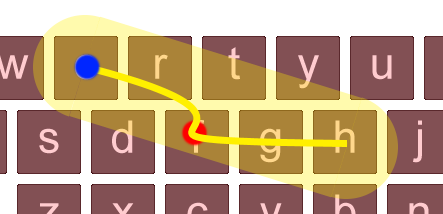
\includegraphics[width=2.5in]{fig_path_with_error}
		\subcaption{Error with Path Protection}
	\end{minipage}
	\caption[Protected Path Example]{A path between the currently pressed letter and the next letter significantly reduces the chance of detecting erroneous input. \textbf{(a)} shows an error detected with an angle less than 165 degrees. \textbf{(b)} shows how as long as the user stays on the path, errors are significantly reduced. \textbf{(c)} shows that errors can still be detected on a protected path if a deviation with an angle less than 90 degrees is detected.}
	\label{protected_path}
\end{figure}

The specific values for detecting key presses were found using trial and error and were used to create an experience as close to a word-gesture keyboard as possible. The main deviation between this implementation and one with word-recognition is that participants are shown updates in real-time of what the keyboard path is doing. This was determined to be an acceptable limitation.

\subsection{Display}
\subsubsection{Keyboard Layout}
The keyboard layout, seen in Figure~\ref{keyboard_layout}, was laid out in a typical QWERTY keyboard fashion with key sizes of 64x64 pixels and gaps of 10 pixels. All special keys and number keys were removed to simplify the keyboard and a backspace key added to the right of the keyboard to allow for deletion of erroneous characters.

\begin{figure}[h]
	\centering
	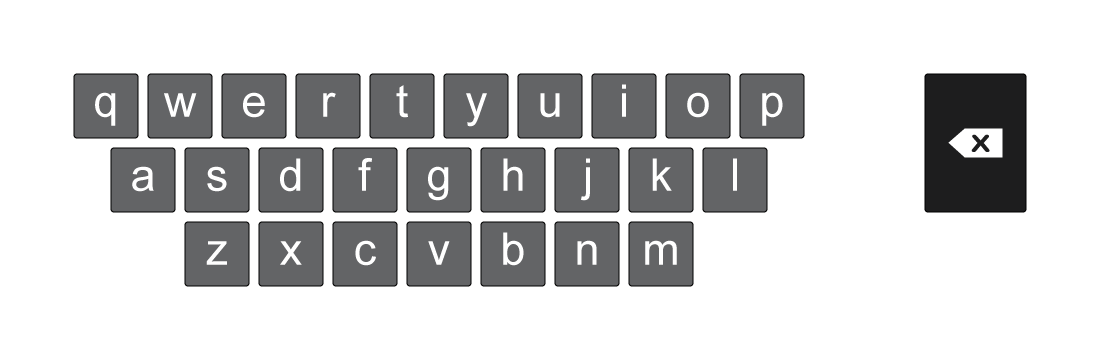
\includegraphics[width=6in]{fig_final_keyboard}
	\caption[Display: Keyboard Layout]{The keyboard layout used during the final study.}
	\label{keyboard_layout}
\end{figure}

\subsubsection{Text Area}
Figure~\ref{text_area} shows how two text areas were used to display text to participants. The top text-area showed the current word to transcribe, shown in Figure~\ref{text_a}, and the bottom area showed the currently transcribed text, shown in Figure~\ref{text_b}. The characters of both the displayed word and transcribed text were highlighted in green when the characters matched and were correct, whereas the letters in only the transcribed text would highlight in red if errors were made during transcription. The participant can then use the back space in order to correct words, and they are finally highlighted in green, as seen in Figure~\ref{text_c}, when a word was completed and correct.

\begin{figure}[b]
	\centering
	\begin{minipage}[t]{1.9in}
		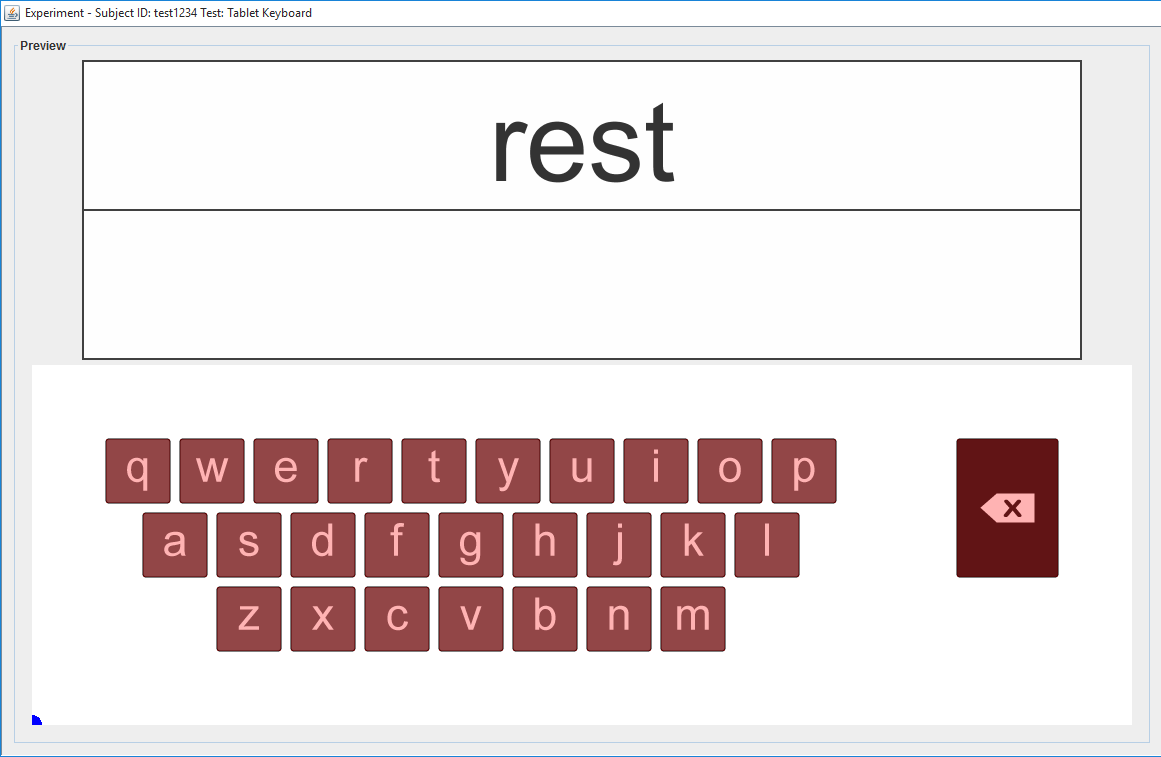
\includegraphics[width=2in]{fig_idle_keyboard}
		\subcaption{Displayed Word}
		\label{text_a}
	\end{minipage}
	\begin{minipage}[t]{1.9in}
		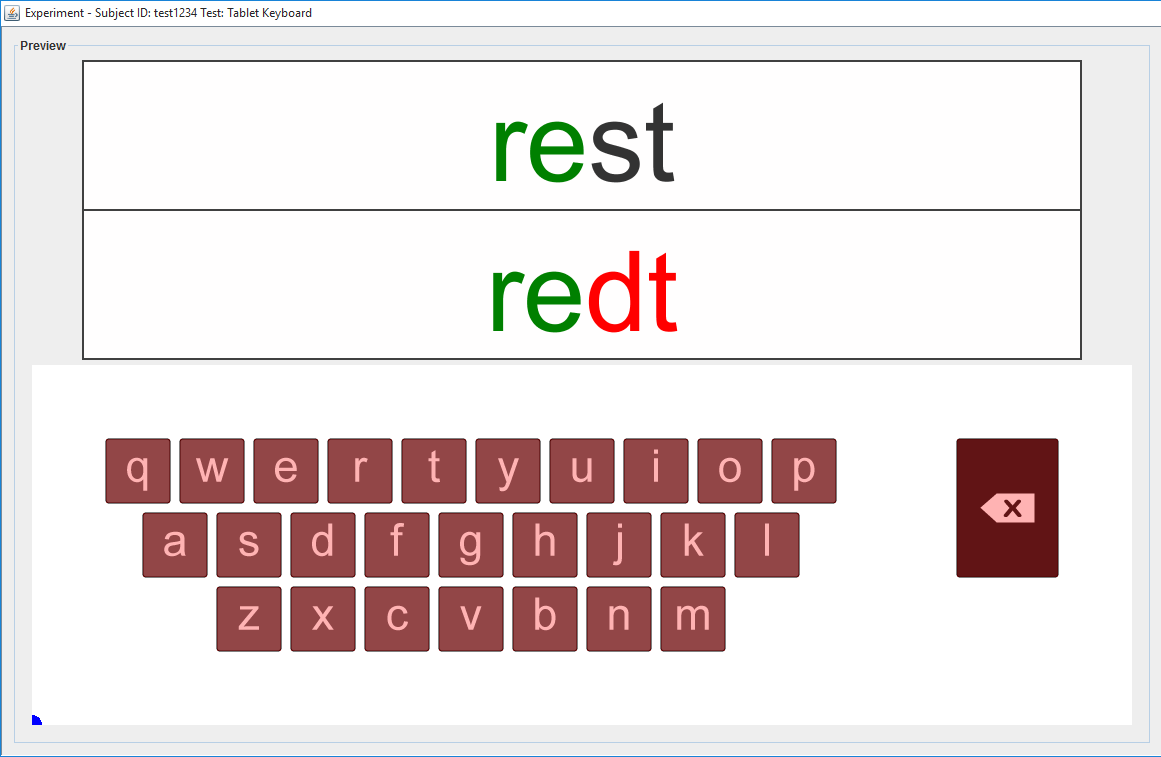
\includegraphics[width=2in]{fig_error_keyboard}
		\subcaption{Transcribed Error}
		\label{text_b}
	\end{minipage}
	\begin{minipage}[t]{1.9in}
		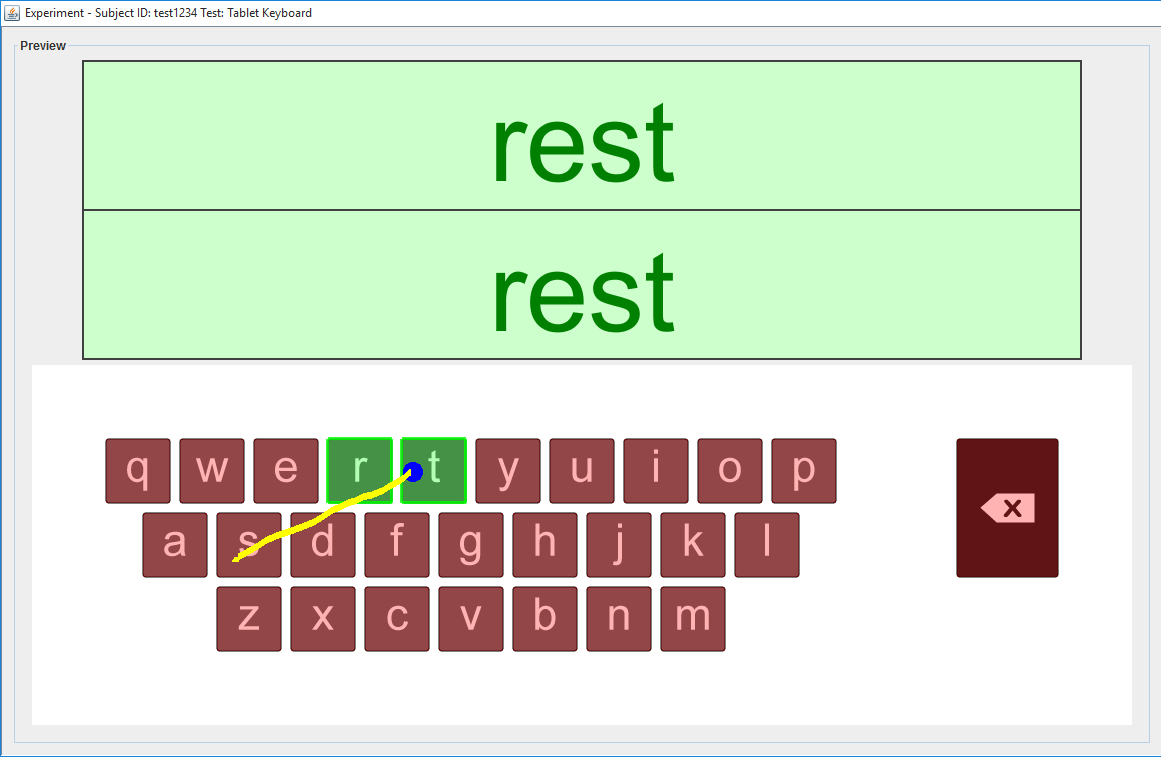
\includegraphics[width=2in]{fig_correct_keyboard}
		\subcaption{Completed Word}
		\label{text_c}
	\end{minipage}
	\caption[Display: Text Area]{Examples of how the text areas change when showing transcribed text. \textbf{(a)} shows the word to transcribe as it first appears. \textbf{(b)} shows how correct letters are highlighted green in both text areas and transcription errors are highlighted in red. \textbf{(c)} shows a completed word; the background lights up to indicate correctness.}
	\label{text_area}
\end{figure}

\subsubsection{Real-Time Updates}
As a participant is drawing the gesture-shape of a word, their progress is tracked in real time, as shown in Figure~\ref{display_area}. For the keyboards that track a participant's finger or the stylus, Figure~\ref{update_a} shows how a cylinder is displayed to indicate the direction that the finger is pointing, as well as which letter is being hovered over, indicated by a blue dot. As in Figure~\ref{update_b}, the participant is shown the path that they are traveling as well as the letters that have been pressed. The gesture-trail has a maximum length before it starts to decay as to not clutter the display. 

\begin{figure}[h]
	\centering
	\begin{minipage}[t]{2.9in}
		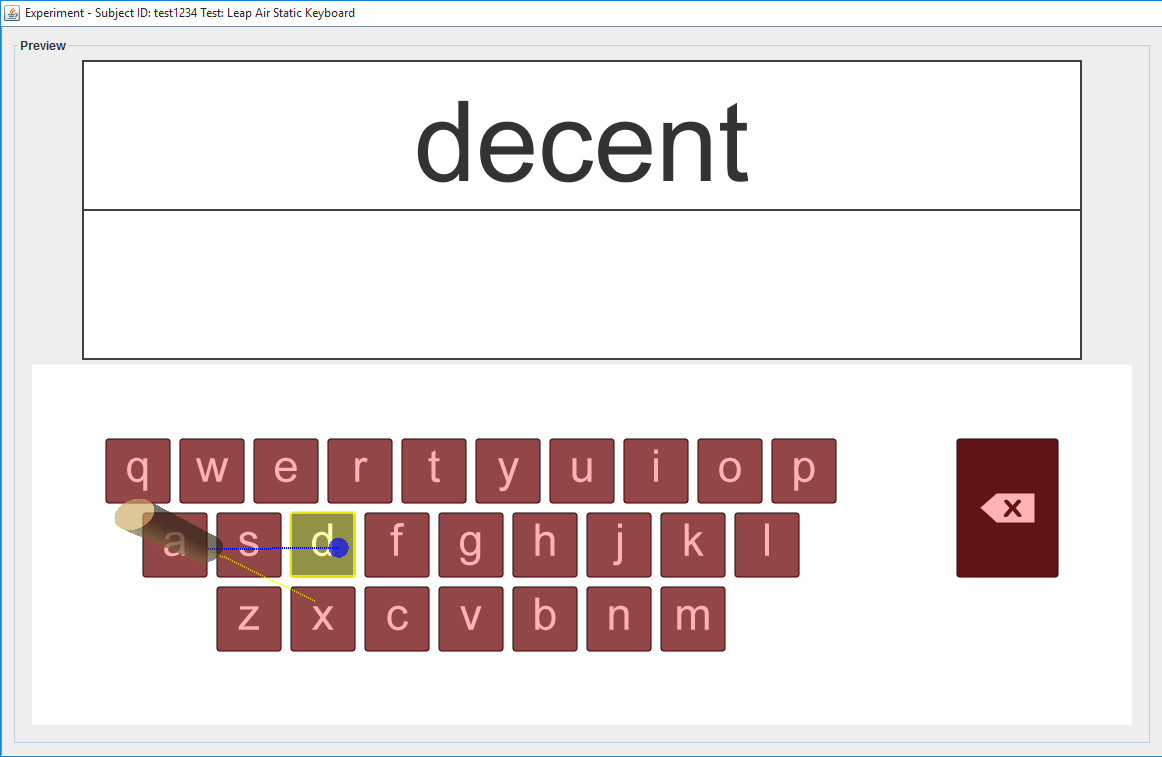
\includegraphics[width=3in]{fig_update1_keyboard}
		\subcaption{Prior to pressing 'd'}
		\label{update_a}
	\end{minipage}
	\begin{minipage}[t]{2.9in}
		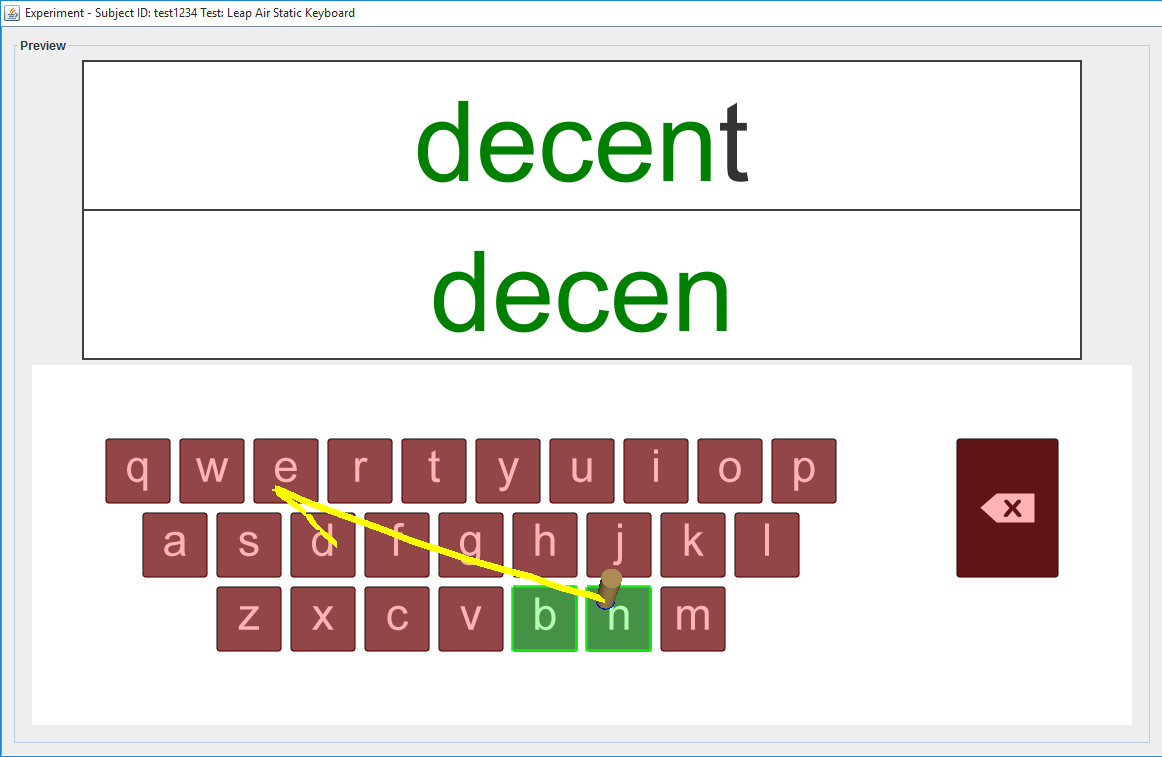
\includegraphics[width=3in]{fig_update2_keyboard}
		\subcaption{During the word-gesture}
		\label{update_b}
	\end{minipage}
	\caption[Display: Real-time Updates]{Examples the real-time display for word-gesturing. \textbf{(a)} shows the user just about to press the first character. \textbf{(b)} shows the middle of the word gesturing process for the word "decent".}
	\label{display_area}
\end{figure}

\subsection{Calibration}
Each mid-air keyboard, including the Leap Surface Keyboard, had the ability to be calibrated in a similar manner as Personal Space \cite{ref_alvin_thesis}, seen in Figure~\ref{calibration_in_progress}. Many of the calibration spaces; however, had to be interacted with directly instead of projecting the participant's hand onto the interaction plane. Calibration was optional and a default calibration was used that worked okay for most people. Calibration had less of a lasting effect because the Leap Motion Controller was allowed to be repositioned which was sometimes a greater factor than the calibration itself. Because this study is not an accessibility study, participants were allowed to calibrate the keyboard with their arms rested or raised, not addressing the "Gorilla Arm Syndrome" mentioned in Section~\ref{gorilla_arm_syndrome}.

\begin{figure}[h]
	\centering
	\begin{minipage}[t]{4in}
		\begin{minipage}[t]{1.9in}
			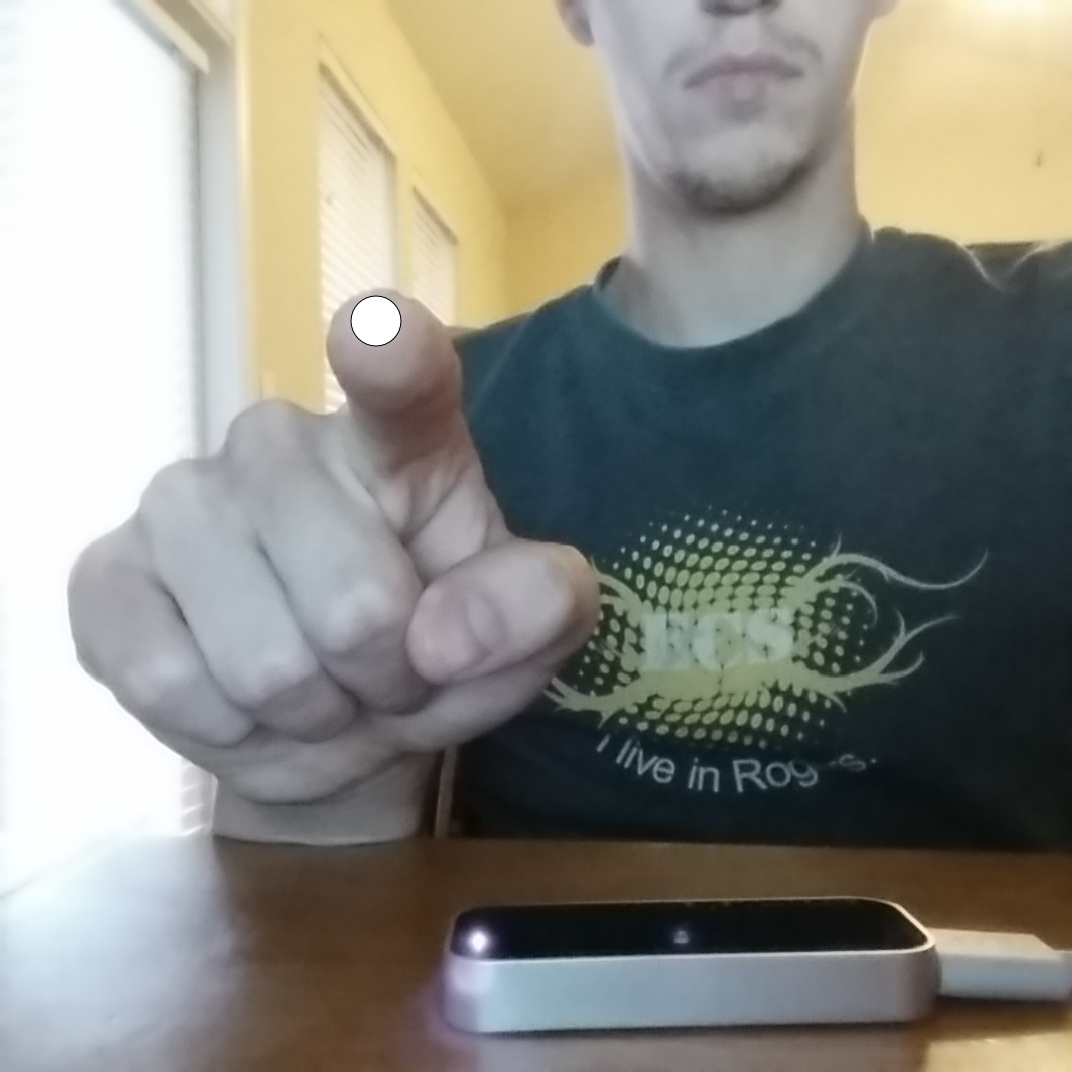
\includegraphics[width=2in]{fig_calib_1}
		\end{minipage}
		\begin{minipage}[t]{1.9in}
			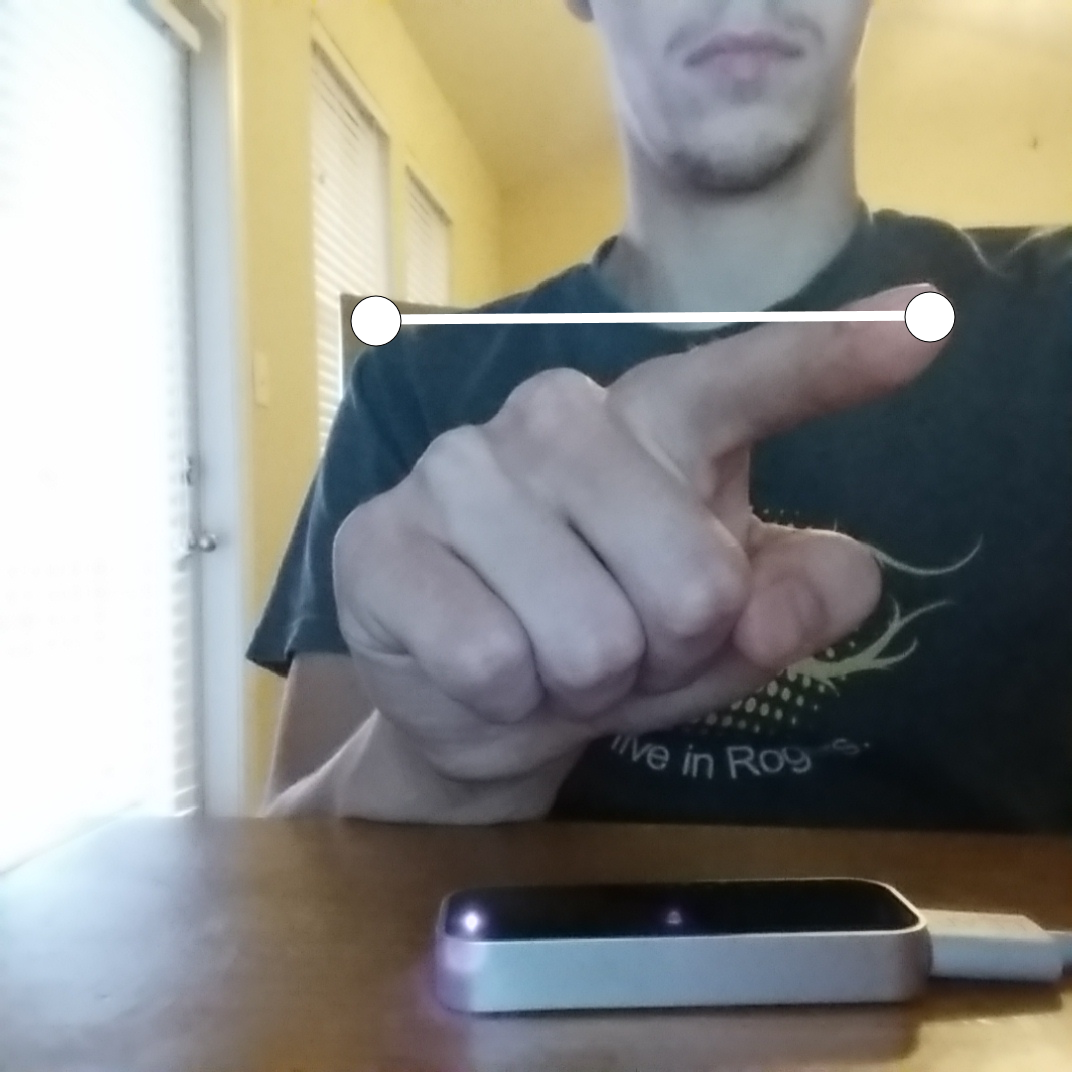
\includegraphics[width=2in]{fig_calib_2}
		\end{minipage}
	\end{minipage}
	
	\begin{minipage}[t]{4in}
		\begin{minipage}[t]{1.9in}
			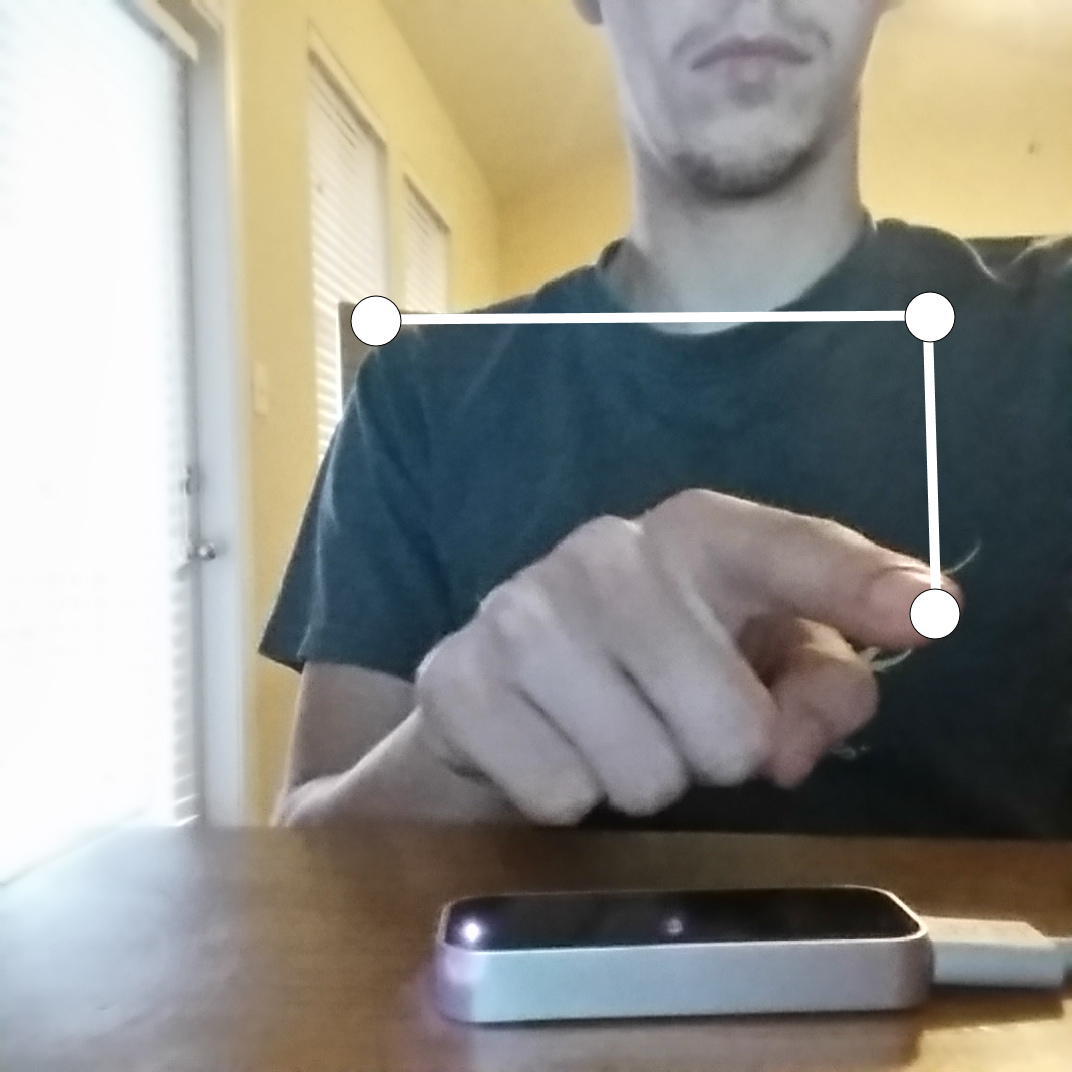
\includegraphics[width=2in]{fig_calib_3}
		\end{minipage}
		\begin{minipage}[t]{1.9in}
			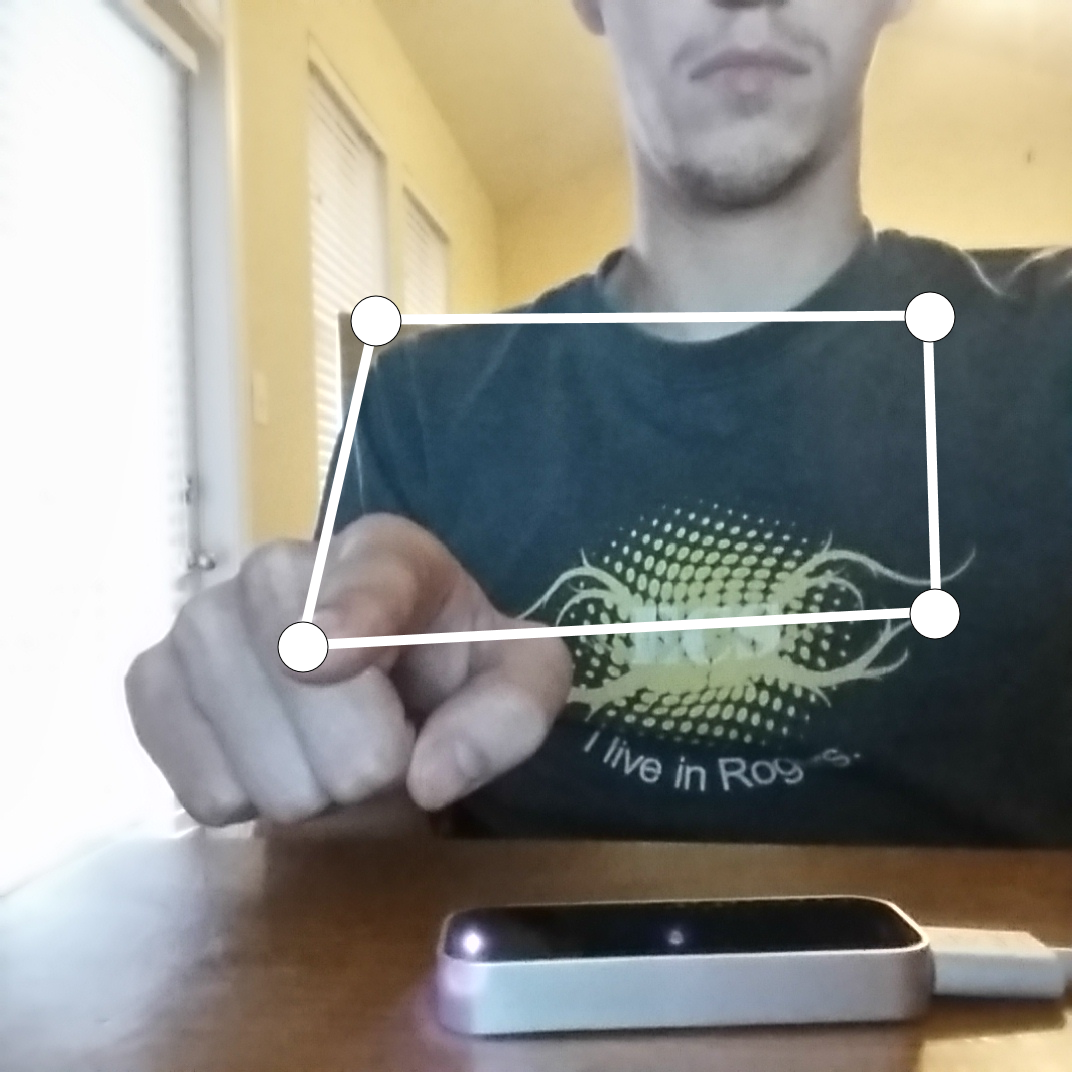
\includegraphics[width=2in]{fig_calib_4}
		\end{minipage}
	\end{minipage}
	\caption[Calibration]{Participants were able to follow on-screen instructions to calibrate the space interaction space using their finger.}
	\label{calibration_in_progress}
\end{figure}

\subsubsection{Motor Space and Display Space}
The calibrated interaction plane, or the motor space, was always attempted to be placed in near parallel to the screen, or display space; however, participants were allowed to move the Leap Motion Controller around to a position that felt best to them. Moving the Leap Motion Controller typically ended up with the motor space being oriented perpendicularly to the participants' arms rather than the display space. Also to note, when working with keyboards that fully utilized the 3rd-Dimension, an interaction plane angled away from the participant was sometimes more effective than a straight plane that was perpendicular to the ground. Figure~\ref{plane_angle} shows the difference between a straight plane and angled plane.

\begin{figure}[h]
	\centering
	\begin{minipage}[t]{4in}
		\begin{minipage}[t]{1.9in}
			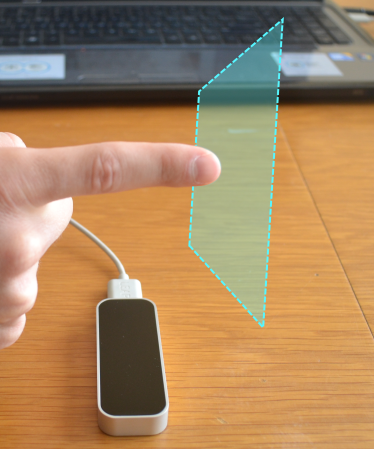
\includegraphics[width=2in]{fig_plane_straight}
			\subcaption{Straight Plane}
		\end{minipage}
		\begin{minipage}[t]{1.9in}
			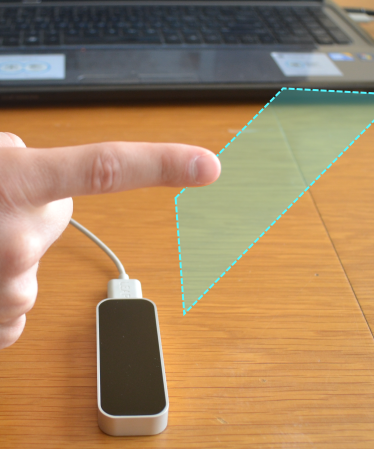
\includegraphics[width=2in]{fig_plane_angled}
			\subcaption{Angled Plane}
		\end{minipage}
	\end{minipage}
	\caption[Angled Plane]{Examples of a straight plane versus an angled plane.}
	\label{plane_angle}
\end{figure}

The size of the motor space was dependent on the device being used or the calibration of the keyboard's interaction plane. For all of the keyboards, the motor space was mapped to a display space with the size of 952x212 pixels and keys that were 64x64 pixels with gaps of 10 pixels. The real-world size of the display was dependent on the screen being used. Figure~\ref{motor_space_size} shows the average sizes of the motor spaces.

\begin{figure}[h]
	\centering
	\begin{minipage}[t]{2.5in}
		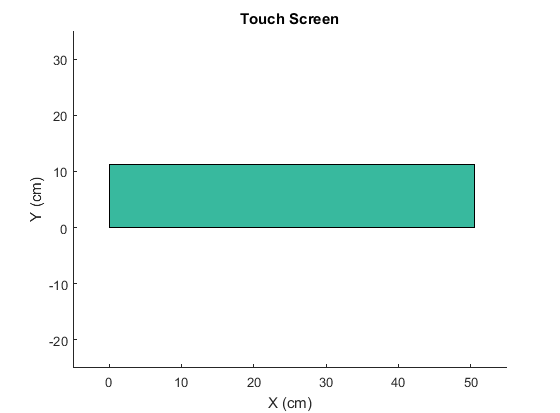
\includegraphics[width=2.5in]{fig_calibration_touch}
		\subcaption{Touch Screen}
		\label{fig_calibration_touch}
	\end{minipage}
	\begin{minipage}[t]{2.5in}
		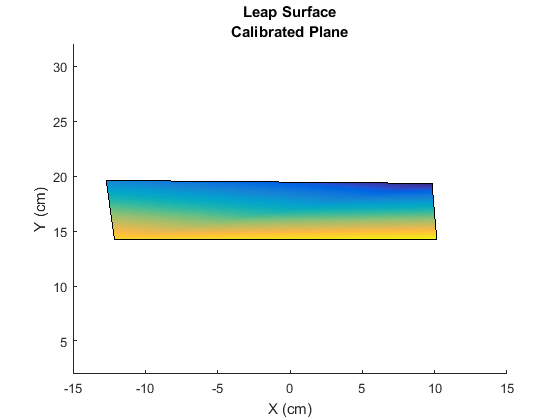
\includegraphics[width=2.5in]{fig_calibration_surface}
		\subcaption{Leap Surface}
		\label{fig_calibration_surface}
	\end{minipage}
	\begin{minipage}[t]{2.5in}
		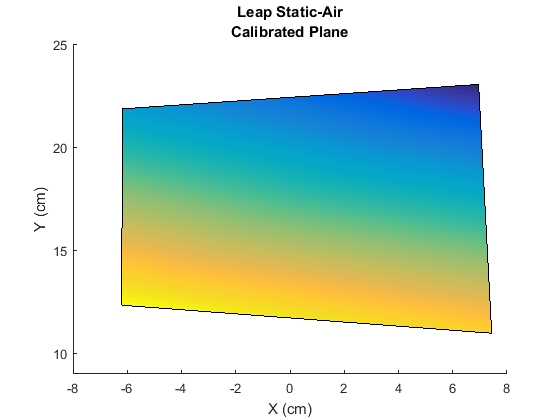
\includegraphics[width=2.5in]{fig_calibration_static}
		\subcaption{Static/Predictive/Bimodal}
		\label{fig_calibration_static}
	\end{minipage}
	\begin{minipage}[t]{2.5in}
		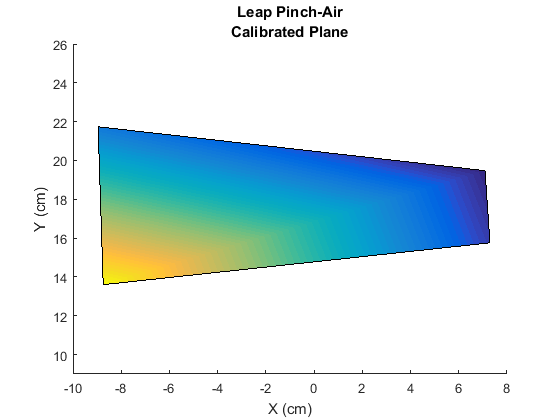
\includegraphics[width=2.5in]{fig_calibration_pinch}
		\subcaption{Leap Pinch-Air}
		\label{fig_calibration_pinch}
	\end{minipage}
	\caption[Motor Space Comparison]{The average size of the motor spaces for each keyboard with a gradient color scale showing the plane orientation. The closest \textbf{yellow} and furthest \textbf{blue}. \textbf{(a)} shows the standard Touch Sceen motor space. \textbf{(b)} shows the average calibration for the Leap Surface motor space. \textbf{(c)} shows the average calibration for the Leap Static-Air, Predictive-Air, and Bimodal-Air motor spaces (typically one was used for all three). \textbf{(d)} shows the average calibration for the Leap Pinch-Air motor space.}
	\label{motor_space_size}
\end{figure}

\subsection{Dictionary Creation} \label{dictionary_creation}
To make each keyboard experience as similar as possible, custom dictionaries were created for each keyboard input device containing words with similar gesture-shapes between keyboards. Dictionaries were created using a custom gesture-shape dissimilarity algorithm. The dictionaries contained words between the character lengths of 3 and 6 so that words would be rather simple, and words that most participants had seen before.

\subsubsection{Using Similar Gesture-Shapes}
The reason that custom dictionaries were chosen to be created was because it was thought that dependent measures would be more accurately represented for each keyboard if the experiences between those keyboards was nearly the same, only changing due to implementation. There was no previous research on words with similar gesture-shapes, or if this was truly necessary or beneficial.

\subsubsection {Gesture-Shape Dissimilarity}
Originally the Fr\'echet Distance was used to try to find the most similar word gesture-shapes using the sets of words with the least distance between each gesture-shape. Fr\'echet Distance gave acceptable results, however there were noticeable differences in some of the paths created.

In order to achieve gesture-shapes with even closer similarity, a custom dissimilarity algorithm to rate words' gesture-shapes of the same length was created. The top results for words with the least dissimilarity between each other were then split among the dictionaries. The dissimilarity between two words is defined by the formula
\begin{equation}
dissimilarity(P,\ Q) = \frac{\sum\limits_{i = 2}^{N} \frac{1}{2} \left(\left(\frac{\mid dist(P_{i},\ P_{i-1}) - dist(Q_{i},\ Q_{i-1})\mid}{max\ distance}\right) + \left(\frac{angle(P_{i} - P_{i-1},\ Q_{i} - Q_{i-1})}{\pi}\right)\right)}{N - 1}
\end{equation}
where $P$ and $Q$ were two words of $N$ length, $P_i$ and $Q_i$ were the vector locations of the characters of the words on the virtual keyboard, $max\ distance$ was the maximum distance between any two letters on the virtual keyboard, $dist(...)$ was the distance between two vector locations, and $angle(...)$ was the angle between two vectors. The dissimilarity formula forced values between the range [0, 1] and treated every pair of paths between two letters of two words with equal weight. The objective was then to find the sets of words with the lowest dissimilarity.

\section{Word-Gesture Keyboards}
All of the word-gesture keyboards created used the same word-gesturing implementation but differentiated by their interaction method and how touch simulation was handled as a delimiter between words.

\subsection{Touch Screen Keyboard}
\subsubsection{Interaction Method}
The Touch Screen Keyboard was implemented to mirror the de facto method for word-gesture keyboards which are touch-based. The user interacts directly with a touch screen surface.

\subsubsection{Word Separation}
Figure~\ref{touch_screen_press_comparison} shows that word separation for the Touch Screen Keyboard worked in the same way as typical word-gesture keyboards for phones and tablets. Touch was simulated simply by pressing a finger against the surface, drawing the word-gesture, and then removing the finger from the surface.

\begin{figure}[h]
	\centering
	\begin{minipage}[t]{5.8in}
		\begin{minipage}[t]{2.85in}
			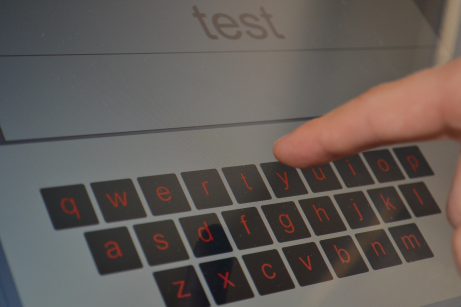
\includegraphics[width=2.9in]{fig_touch_screen_hover}
		\end{minipage}
		\begin{minipage}[t]{2.9in}
			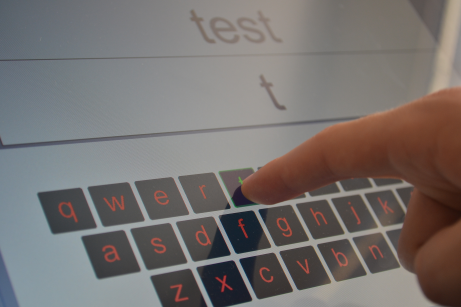
\includegraphics[width=2.9in]{fig_touch_screen_press}
		\end{minipage}
	\end{minipage}
	\caption[Touch Screen Word Separation]{A touch is simulated when the tabletop screen is touched.}
	\label{touch_screen_press_comparison}
\end{figure}

\subsubsection{Size of the Motor Space}
The motor space for the Touch Screen Keyboard was larger than the other keyboards because it utilized the Ideum Multi-touch Table Platform 46" tabletop, shown in Figure~\ref{fig_ideum}, which had a maximum resolution of 1920x1080 pixels. When scaled for the maximum resolution, the Touch Screen display space and motor space were both 50.49x11.24 $cm$, with keys that were 3.39x3.39 $cm$ and gaps between keys of 0.53 $cm$. If higher resolutions were available, a higher resolution would have been chosen to decrease the overall size of the display space and motor space to match the other keyboards more closely. Though larger than desired, the Ideum Multi-touch Table Platform was still preferred over using very small touch-keyboards such as those on phones or tablets. Having similar sized motor spaces was to help standardize results between touch and mid-air.

\begin{figure}[h]
	\centering
	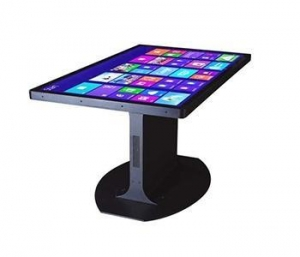
\includegraphics{fig_ideum}
	\caption[Ideum Multi-touch Table Platform]{The Ideum Multi-touch Table Platform tabletop.}
	\label{fig_ideum}
\end{figure}

\subsection{Leap Surface Keyboard} \label{leap_surface}
\subsubsection{Interaction Method}
The Leap Surface Keyboard used the Leap Motion Controller to track a wooden stylus for interaction. It was designed so that it would simulate a touch screen using a mid-air plane projected onto a surface. This was done by inserting the Leap Motion into a custom holder, shown in Figure~\ref{fig_leap_holder}, and projecting the mid-air keyboard over a keyboard printed on paper. As an added note, the Leap Surface Keyboard works in the exact same way as the Static-Air Keyboard in Section~\ref{static_air} except for that it is calibrated to a surface rather than mid-air. A stylus was chosen to be used as an interaction tool for this setup to allow for accurate surface emulation because the Leap Motion Controller was in a position that made it difficult to successfully track a participants hand or finger. Unfortunately, the Leap Controller had to be positioned in the way that it was because the hardware, at the time of implementation, was not designed to recognize hands from the other direction, or otherwise "upsidedown".

\begin{figure}[h]
	\centering
	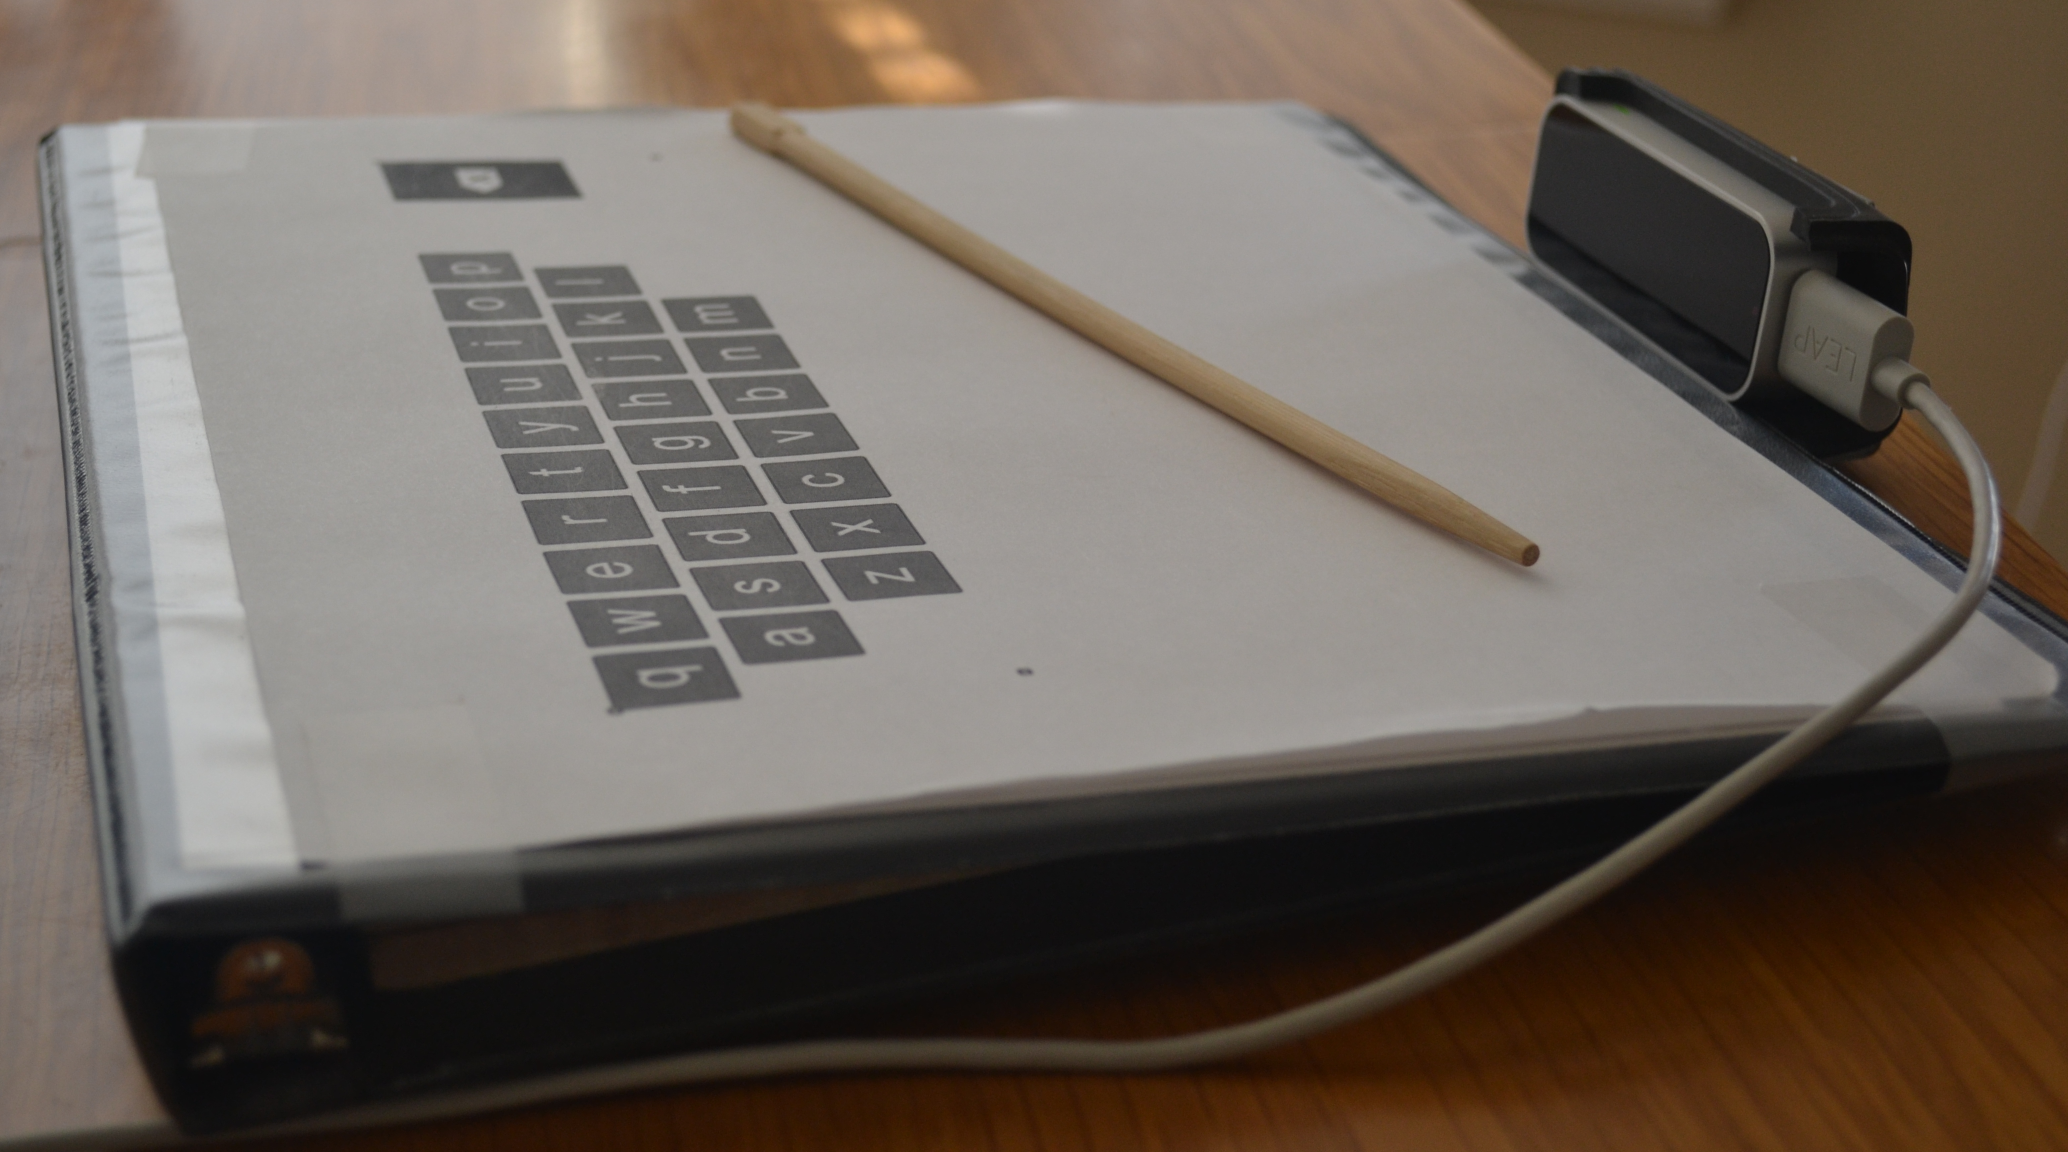
\includegraphics[width=5in]{fig_leap_holder}
	\caption[Leap Surface Holder]{The custom built holder, projecting an interaction plane onto a printed keyboard surface.}
	\label{fig_leap_holder}
\end{figure}

\subsubsection{Word Separation}
Word separation for the Leap Surface Keyboard worked in a similar way to how touch is simulated using a stylus for a phone or tablet. Figure~\ref{leap_surface_press_comparison} shows how touch was simulated by pressing the tip of the stylus against the surface of the printed keyboard. The word-gestures was drawn and then the stylus removed from the surface to complete the action.

\begin{figure}[h]
	\centering
	\begin{minipage}[t]{5.8in}
		\begin{minipage}[t]{2.85in}
			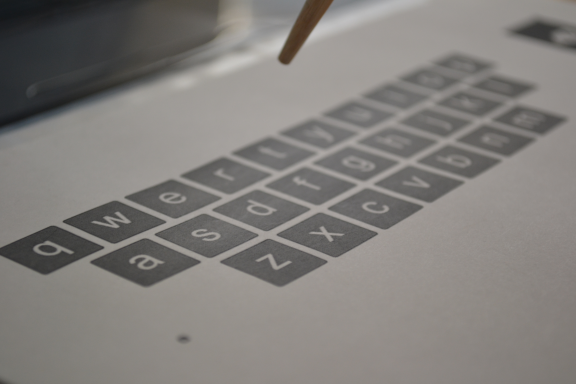
\includegraphics[width=2.9in]{fig_surface_hover}
		\end{minipage}
		\begin{minipage}[t]{2.9in}
			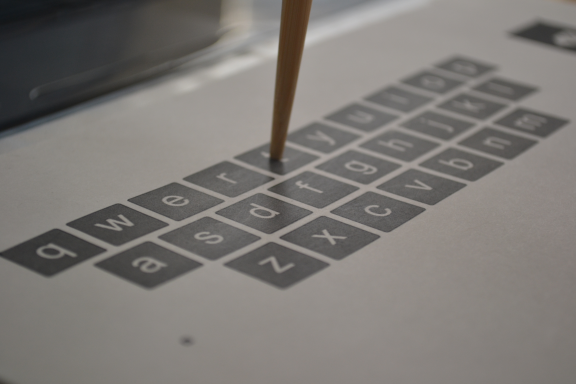
\includegraphics[width=2.9in]{fig_surface_touch}
		\end{minipage}
	\end{minipage}
	\caption[Leap Surface Word Separation]{A touch is simulated when the stylus hits the paper surface.}
	\label{leap_surface_press_comparison}
\end{figure}

\subsubsection{Size of the Motor Space}
Figure~\ref{fig_calibration_surface} shows the average calibrated motor space for the Leap Surface Keyboard. The average keyboard was 22.28x5.41 $cm$, with keys that were 1.50x1.50 $cm$ and gaps between keys of 0.23 $cm$.

\subsection{Leap Static-Air Keyboard} \label{static_air}
\subsubsection{Interaction Method}
The Leap Static-Air Keyboard used the Leap Motion Controller to track the pointer finger of either hand for interaction. It was designed so that it would simulate a touch screen in mid-air by projecting a quadrilateral plane in the air. The pointer finger would then be used to penetrate the plane to simulate touch.

\subsubsection{Word Separation}
Word separation for the Leap Static-Air Keyboard worked in a similar way as any ordinary touch-based word-gesture keyboard, however the simulated touch plane was in mid-air. Touch was simulated by using either pointer finger and penetrating the mid-air interaction plane as seen in Figure~\ref{static_press_comparison}. Then while maintaining the intersection, the pointer finger was used to draw the word-gesture, and then finally by pulling the finger away from the mid-air interaction plane, touch was released.

\begin{figure}[h]
	\centering
	\begin{minipage}[t]{5.8in}
		\begin{minipage}[t]{2.85in}
			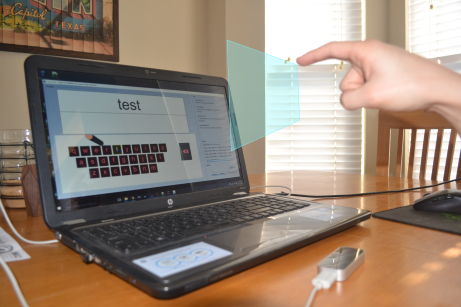
\includegraphics[width=2.9in]{fig_static_hover}
		\end{minipage}
		\begin{minipage}[t]{2.9in}
			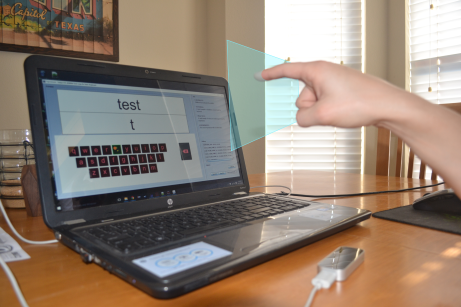
\includegraphics[width=2.9in]{fig_static_touch}
		\end{minipage}
	\end{minipage}
	\caption[Leap Static-Air Word Separation]{A touch is simulated by penetrating the interaction plane.}
	\label{static_press_comparison}
\end{figure}

\subsubsection{Size of the Motor Space}
Figure~\ref{fig_calibration_static} shows the average calibrated motor space for the Leap Static-Air Keyboard. The average keyboard was 13.71x10.07 $cm$, with keys that were 0.92x0.92 $cm$ and gaps between keys of 0.14 $cm$, the same as the Predictive-Air and Bimodal-Air keyboards.

\subsection{Leap Predictive-Air Keyboard}
\subsubsection{Interaction Method}
The Leap Predictive-Air Keyboard used the Leap Motion Controller to track the pointer finger of either hand for interaction. It was designed so that it would simulate a touch screen in mid-air by projecting a quadrilateral plane in the air; however, instead of having to interact with a static, unchanging plane, the Predictive-Air Keyboard associates the interaction plane with the participant's pointer finger. As the pointer finger moves forward or backward, the plane follows. The Predictive-Air Keyboard then tries to move the interaction plane to the pointer finger by predicting when a touch is being simulated by analyzing forward and backward hand gestures. Slow gestures serve mostly to move the plane, whereas quick gestures generally snap the pointer finger to the plane. The implementation of the forward and backward hand gestures are received from the base Leap Motion API.

\subsubsection{Word Separation}
Word separation for the Predictive-Air Keyboard worked in a similar way as any ordinary touch-based word-gesture keyboard, however the simulated touch plane is in mid-air. The mid-air interaction plane was kept at a static distance away from the detected pointer finger until a forward hand gesture was detected to simulate a touch. Once a touch was simulated, the pointer finger can then be used to draw the word-gesture until it is completed. Finally by making a backward hand gesture away from the interaction plane, the simulated touch is released. The plane interaction is visually similar to Figure~\ref{static_press_comparison}, the Leap Static-Air Keyboard interaction.

\subsubsection{Size of the Motor Space}
Figure~\ref{fig_calibration_static} shows the average calibrated motor space for the Leap Predictive-Air Keyboard. The average keyboard was 13.71x10.07 $cm$, with keys that were 0.92x0.92 $cm$ and gaps between keys of 0.14 $cm$, the same as the Static-Air and Bimodal-Air keyboards.

\subsection{Leap Bimodal-Air Keyboard}
\subsubsection{Interaction Method}
The Leap Bimodal-Air Keyboard used the Leap Motion Controller to track the pointer finger of either hand for interaction. It was designed by projecting a quadrilateral plane in the air and snapping the movements of the pointer finger to that plane. A touch was simulated by using a secondary input, in this case, a standard keyboard's space bar key.

\subsubsection{Word Separation}
Word separation for the Leap Bimodal-Air Keyboard worked by using a secondary input, the space bar. The interaction plane for simulated touch, as seen in Figure~\ref{bimodal_press}, was still projected in mid-air. Touch was simulated by using either pointer finger to determine the position over the interaction plane in the $x$-direction and $y$-direction and then by pressing and holding the space bar key to simulate touch. Then, while holding down the space bar, the pointer finger was used to draw the word-gesture and finally the space bar was released to end the touch.

\begin{figure}[h]
	\centering
	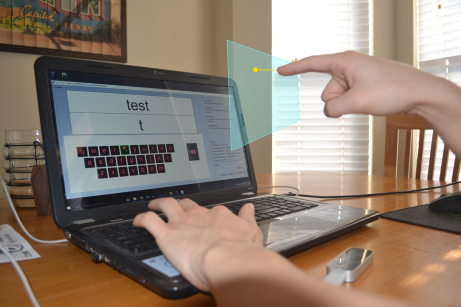
\includegraphics[width=5in]{fig_leap_bimodal}
	\caption[Leap Bimodal-Air Word-Separation]{A touch is simulated simply by pressing the space bar on the keyboard.}
	\label{bimodal_press}
\end{figure}

\subsubsection{Size of the Motor Space}
Figure~\ref{fig_calibration_static} shows the average calibrated motor space for the Leap Bimodal-Air Keyboard. The average keyboard was 13.71x10.07 $cm$, with keys that were 0.92x0.92 $cm$ and gaps between keys of 0.14 $cm$, the same as the Static-Air and Bimodal-Air keyboards.

\subsection{Leap Pinch-Air Keyboard}
\subsubsection{Interaction Method}
The Leap Pinch-Air Keyboard used the Leap Motion Controller to track the palm of either hand for interaction. It was designed in mid-air by projecting a quadrilateral plane in the air and snapping the palm position to the plane in the $z$-direction. The hand then could be used to form a pinch-gesture to simulate touch. The implementation of the pinch-gestures are received from the base Leap Motion API. It is important to note that unlike in Vulture \cite{ref_vulture}, no glove is required and many different pinch-gestures are recognized.

\subsubsection{Word Separation}
Word separation for the Leap Pinch-Air Keyboard worked by using a pinching-gesture; however, the interaction plane was still projected in mid-air. Touch was simulated by using either hand and then forming and holding a pinching-gesture, as shown in Figure~\ref{pinch_press_comparison}. While pinching, the word-gesture was drawn and then the pinching-gesture was released to end the touch.

\begin{figure}[h]
	\centering
	\begin{minipage}[t]{5.8in}
		\begin{minipage}[t]{2.85in}
			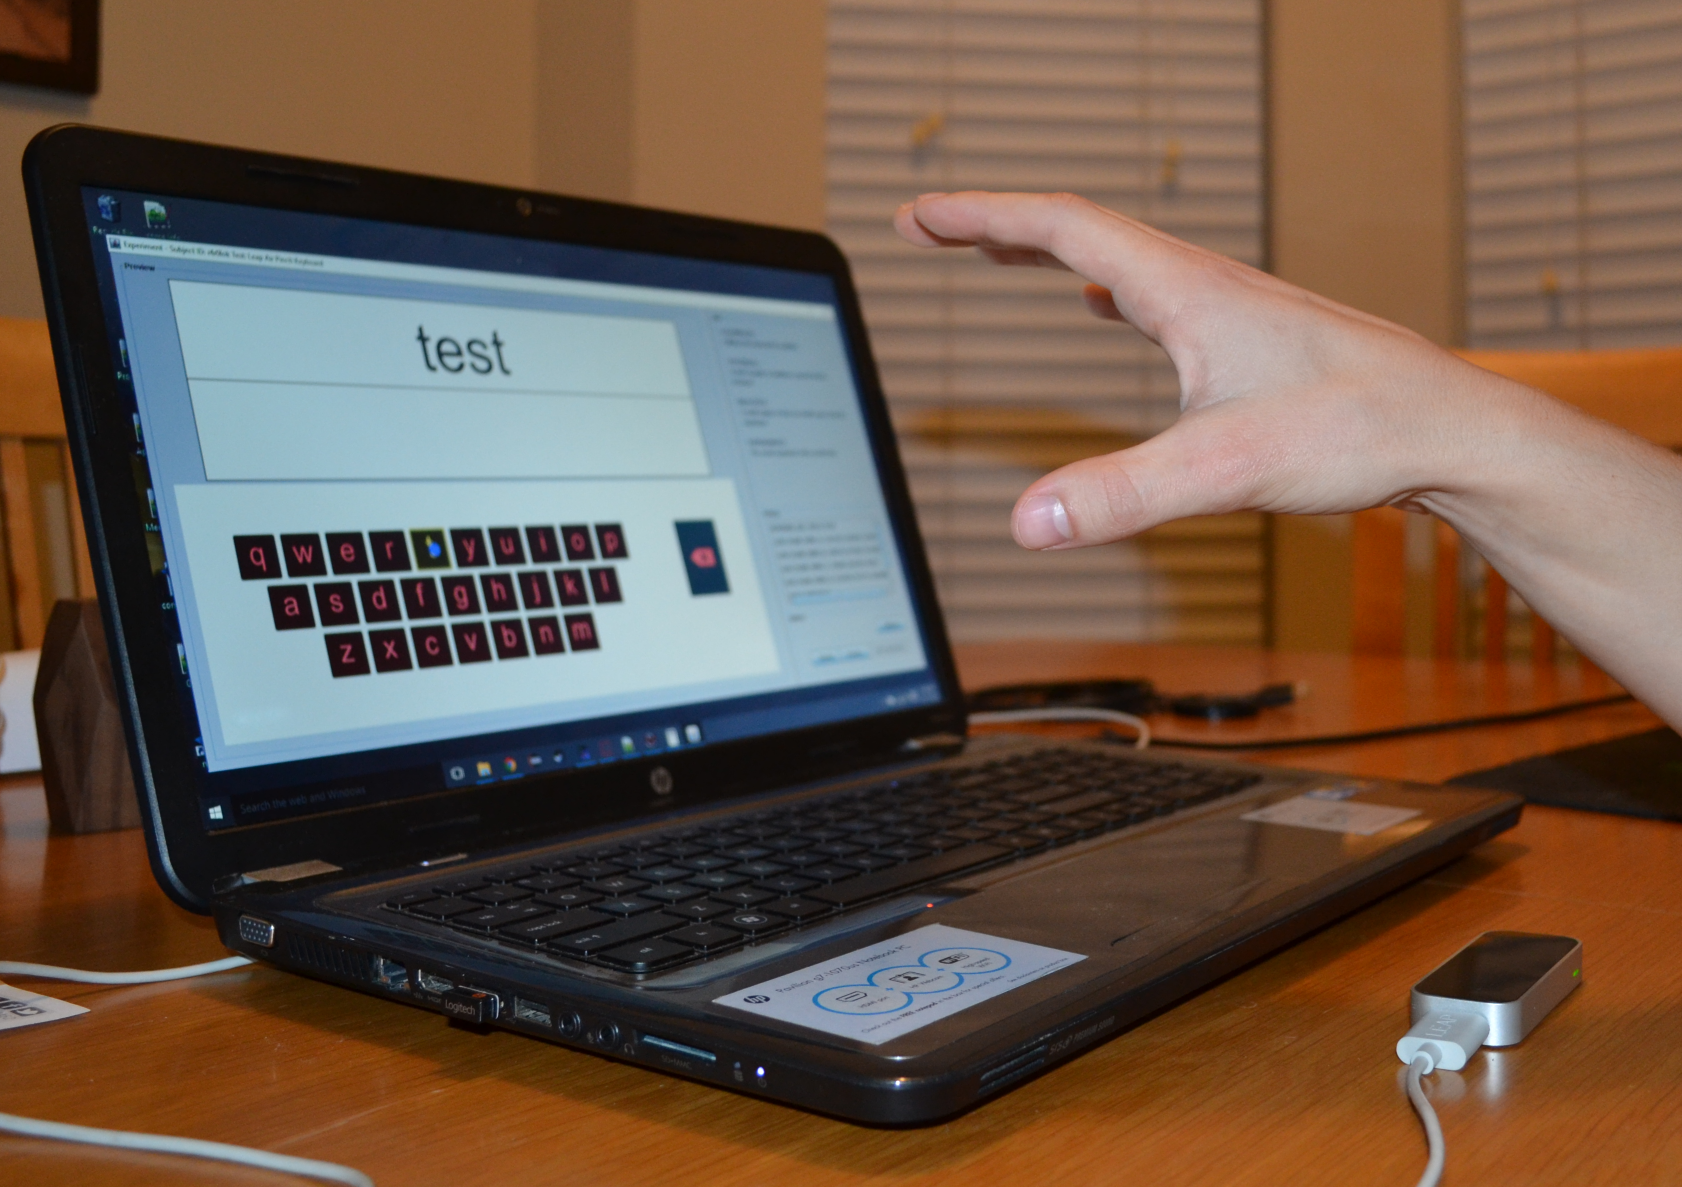
\includegraphics[width=2.9in]{fig_pinch_hover}
		\end{minipage}
		\begin{minipage}[t]{2.9in}
			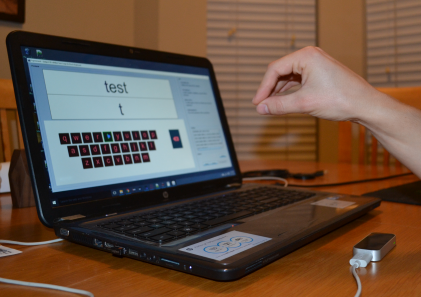
\includegraphics[width=2.9in]{fig_pinch_touch}
		\end{minipage}
	\end{minipage}
	\caption[Leap Pinch-Air Word Separation]{A touch is simulated by making a pinching gesture.}
	\label{pinch_press_comparison}
\end{figure}

\subsubsection{Size of the Motor Space}
Figure~\ref{fig_calibration_pinch} shows the average calibrated motor space for the Leap Pinch-Air Keyboard. The average keyboard was 16.86x9.04 $cm$, with keys that were 1.13x1.13 $cm$ and gaps between keys of 0.18 $cm$.